\section{Results}

\subsection{Level-3 data of Chlorophyll-a Concentration in the East Sea (Sea of Japan).}

Figure \ref{fig:monLAC01}. - Figure \ref{fig:monGAC03}\ are 1km-resolution monthly-mean data of chlorophyll-a Level-3 data in the study area which is 34.00°N - 44.00°N, 127.00°E - 135.00°E. These kinds of Level-3 data are useful for sensing temporal distribution of chlorophyll-a at a specific location. The monthly-mean chlorophyll-a concentration of the LAC data from 2003 to 2006 is shown in Figure \ref{fig:monLAC01}. - Figure \ref{fig:monLAC03}, and the monthly-mean chlorophyll-a concentration of the GAC data from 2003 to 2006 is shown in Figure \ref{fig:monGAC01} - Figure \ref{fig:monGAC03}.
In these figures, the gray area is land of the eastern part of Korea and the southwestern part of Japan. Chlorophyll-a concentrations in the sea were expressed in color. The yellow color indicate about 1 ${\rm mg/m^3}$ and the red color indicate about 10 ${\rm mg/m^3}$ as it is shown at the color bar which is in a logarithm scale. Spring (March, April) and fall (October, November) show high concentration. 

The black area is part with no data due to cloud coverage or satellite failures. LAC data in 2005 especially show large black areas because less files had been aggeragated compared to other years. The black areas in Winter (January, December) can also been noticed to be larger than other years and this is caused by cloud coverage.

High chlorophyll-a concentration was observed at Wonsan, Vladivostok, and Pohang. Wonsan showed high concentration on most of the months, except on May and June. Vladivostok had high concentrations on spring(March, April) and fall (October, November) when the overall concentration was high. Pohang showed a chlorophyll-a tail caused by sea current. It occurred quite randomly, and it could be observed well on September to November, 2003. 

Both the LAC and the GAC data showed similar chlorophyll-a distribution, meaning that they are suitable for sensing spatial and temporal distribution of chlorophyll-a concentration.

\begin{figure}[h]
	\centering
	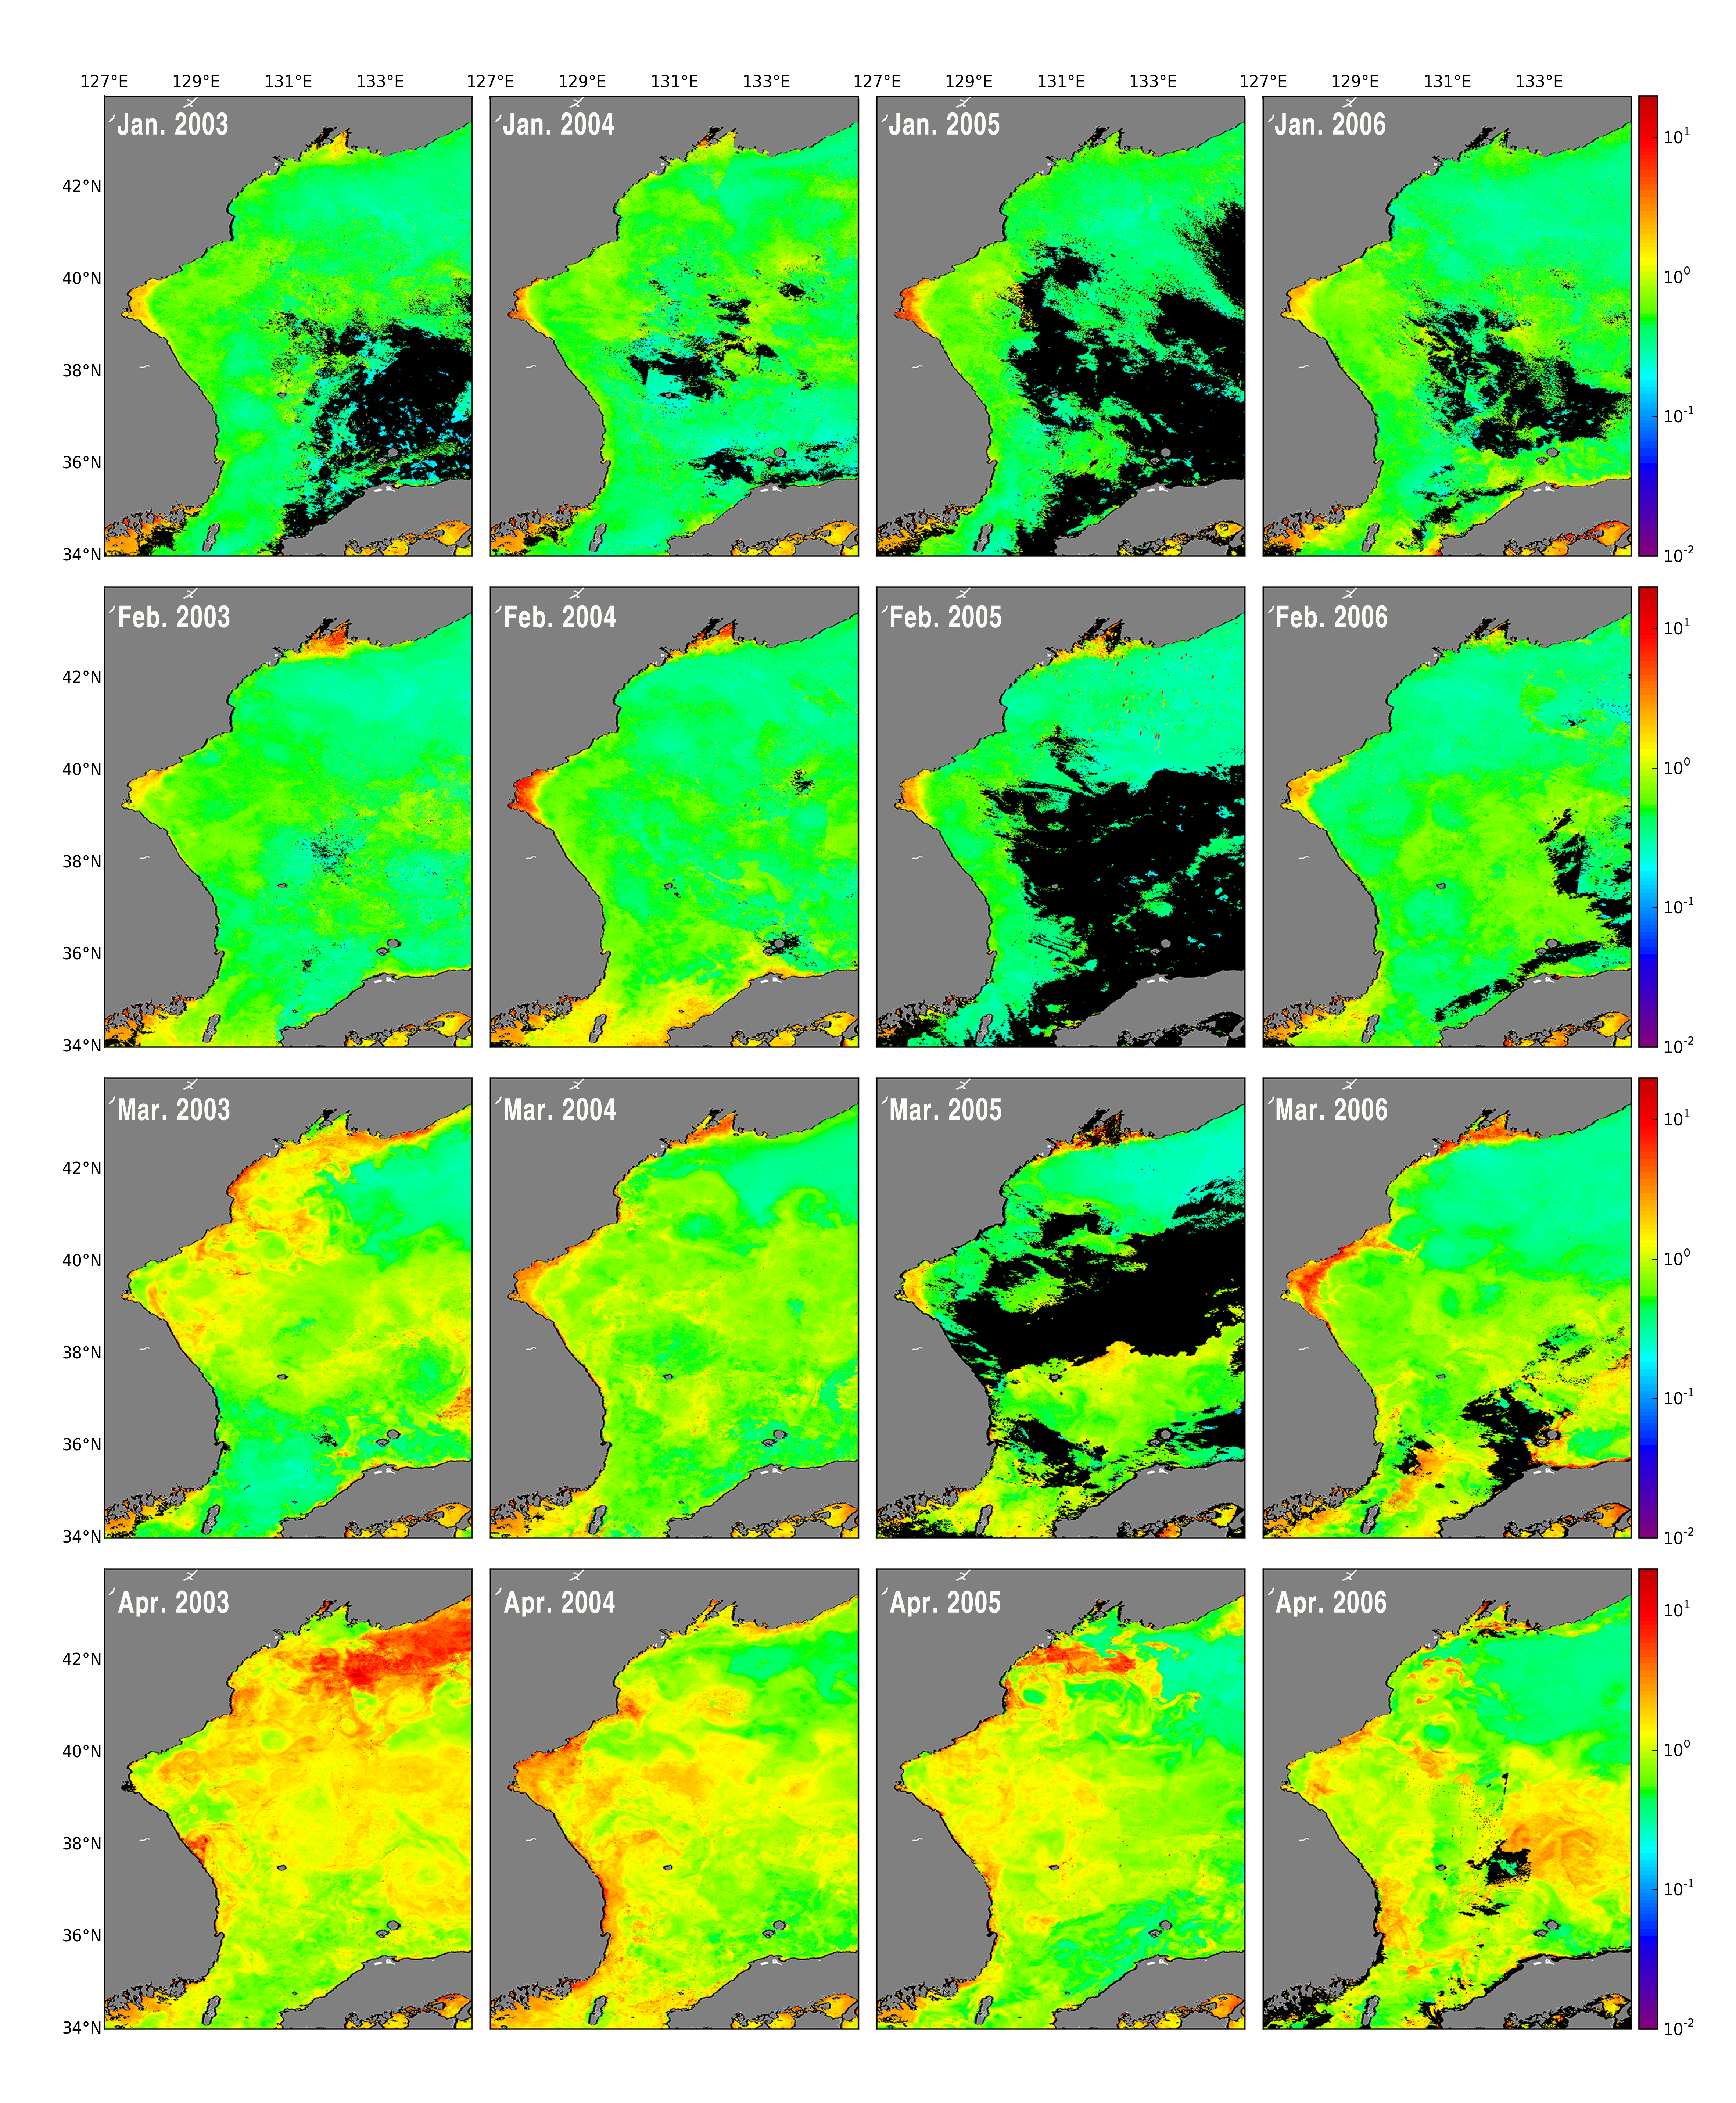
\includegraphics[width=1.0\textwidth]{monLAC01}\\
	\caption{The monthly-mean chlorophyll-a distribution in the East Sea (Sea of Japan), LAC. From 2003 to 2006, January to April.}
	\label{fig:monLAC01}
\end{figure}


\begin{figure}[h]
	\centering
	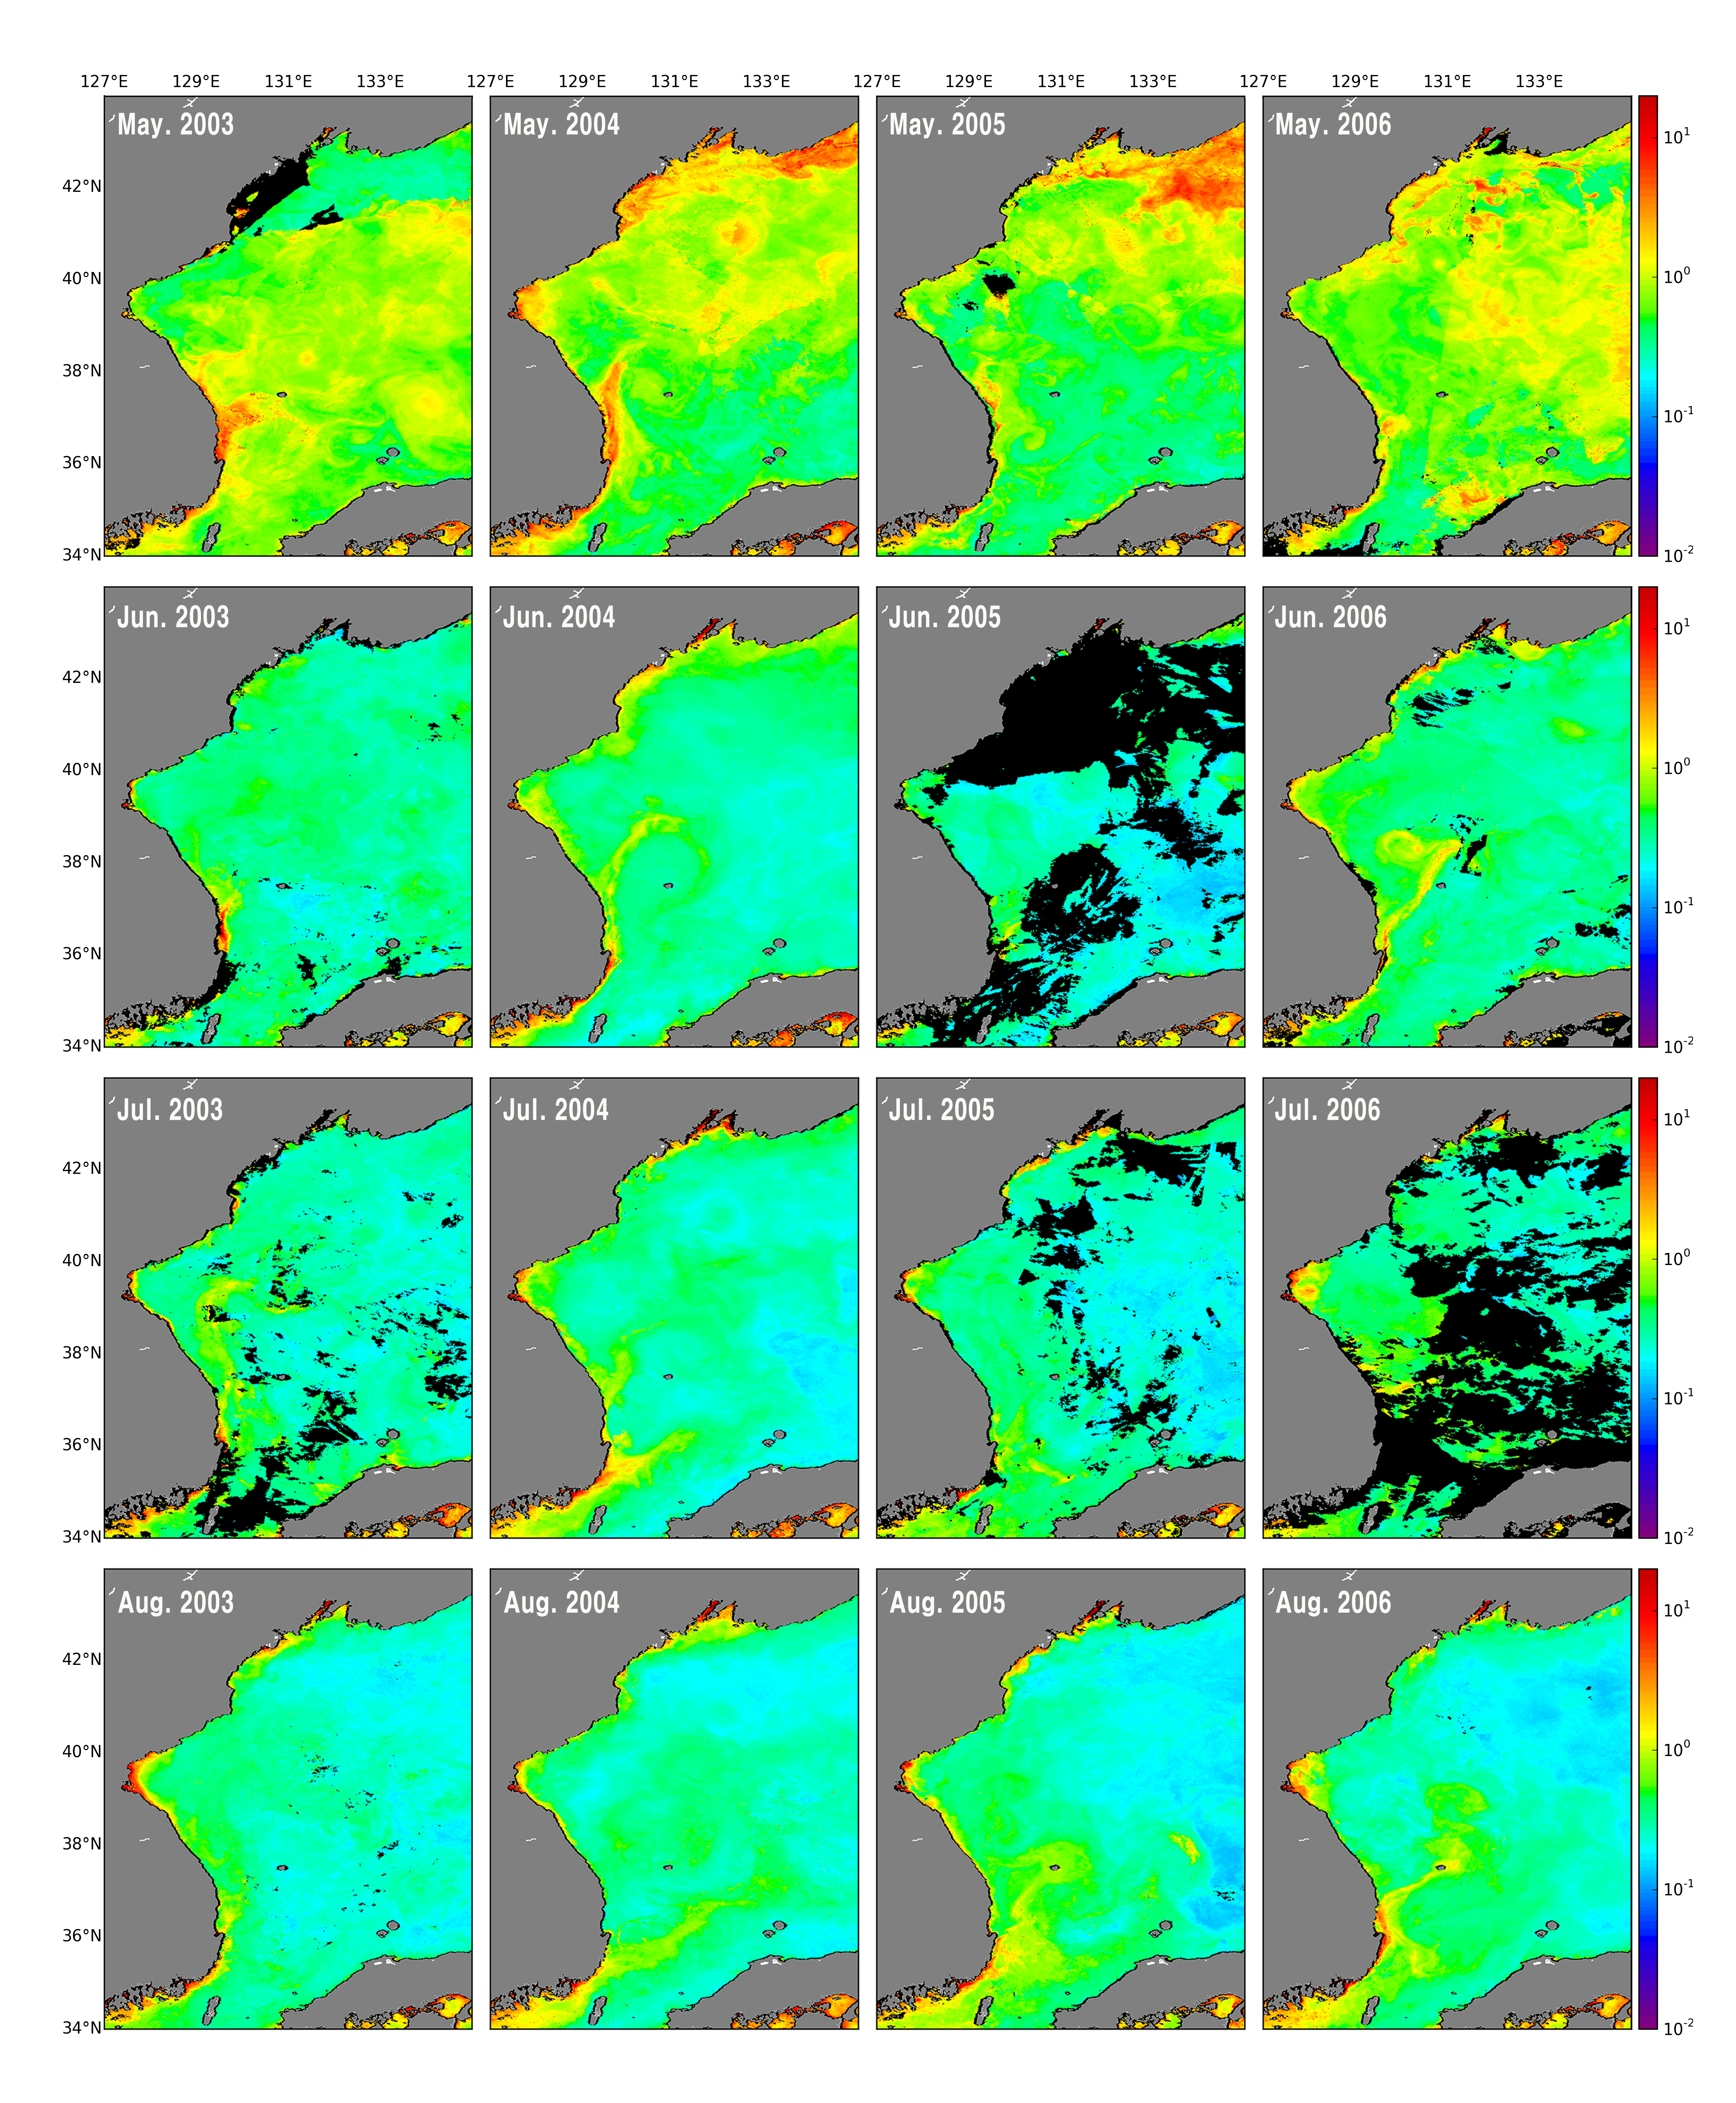
\includegraphics[width=1.00\textwidth]{monLAC02}\\
	\caption{The monthly-mean chlorophyll-a distribution in the East Sea (Sea of Japan), LAC. From 2003 to 2006, May to August.}
	\label{fig:monLAC02}
\end{figure}

\begin{figure}[h]
	\centering
	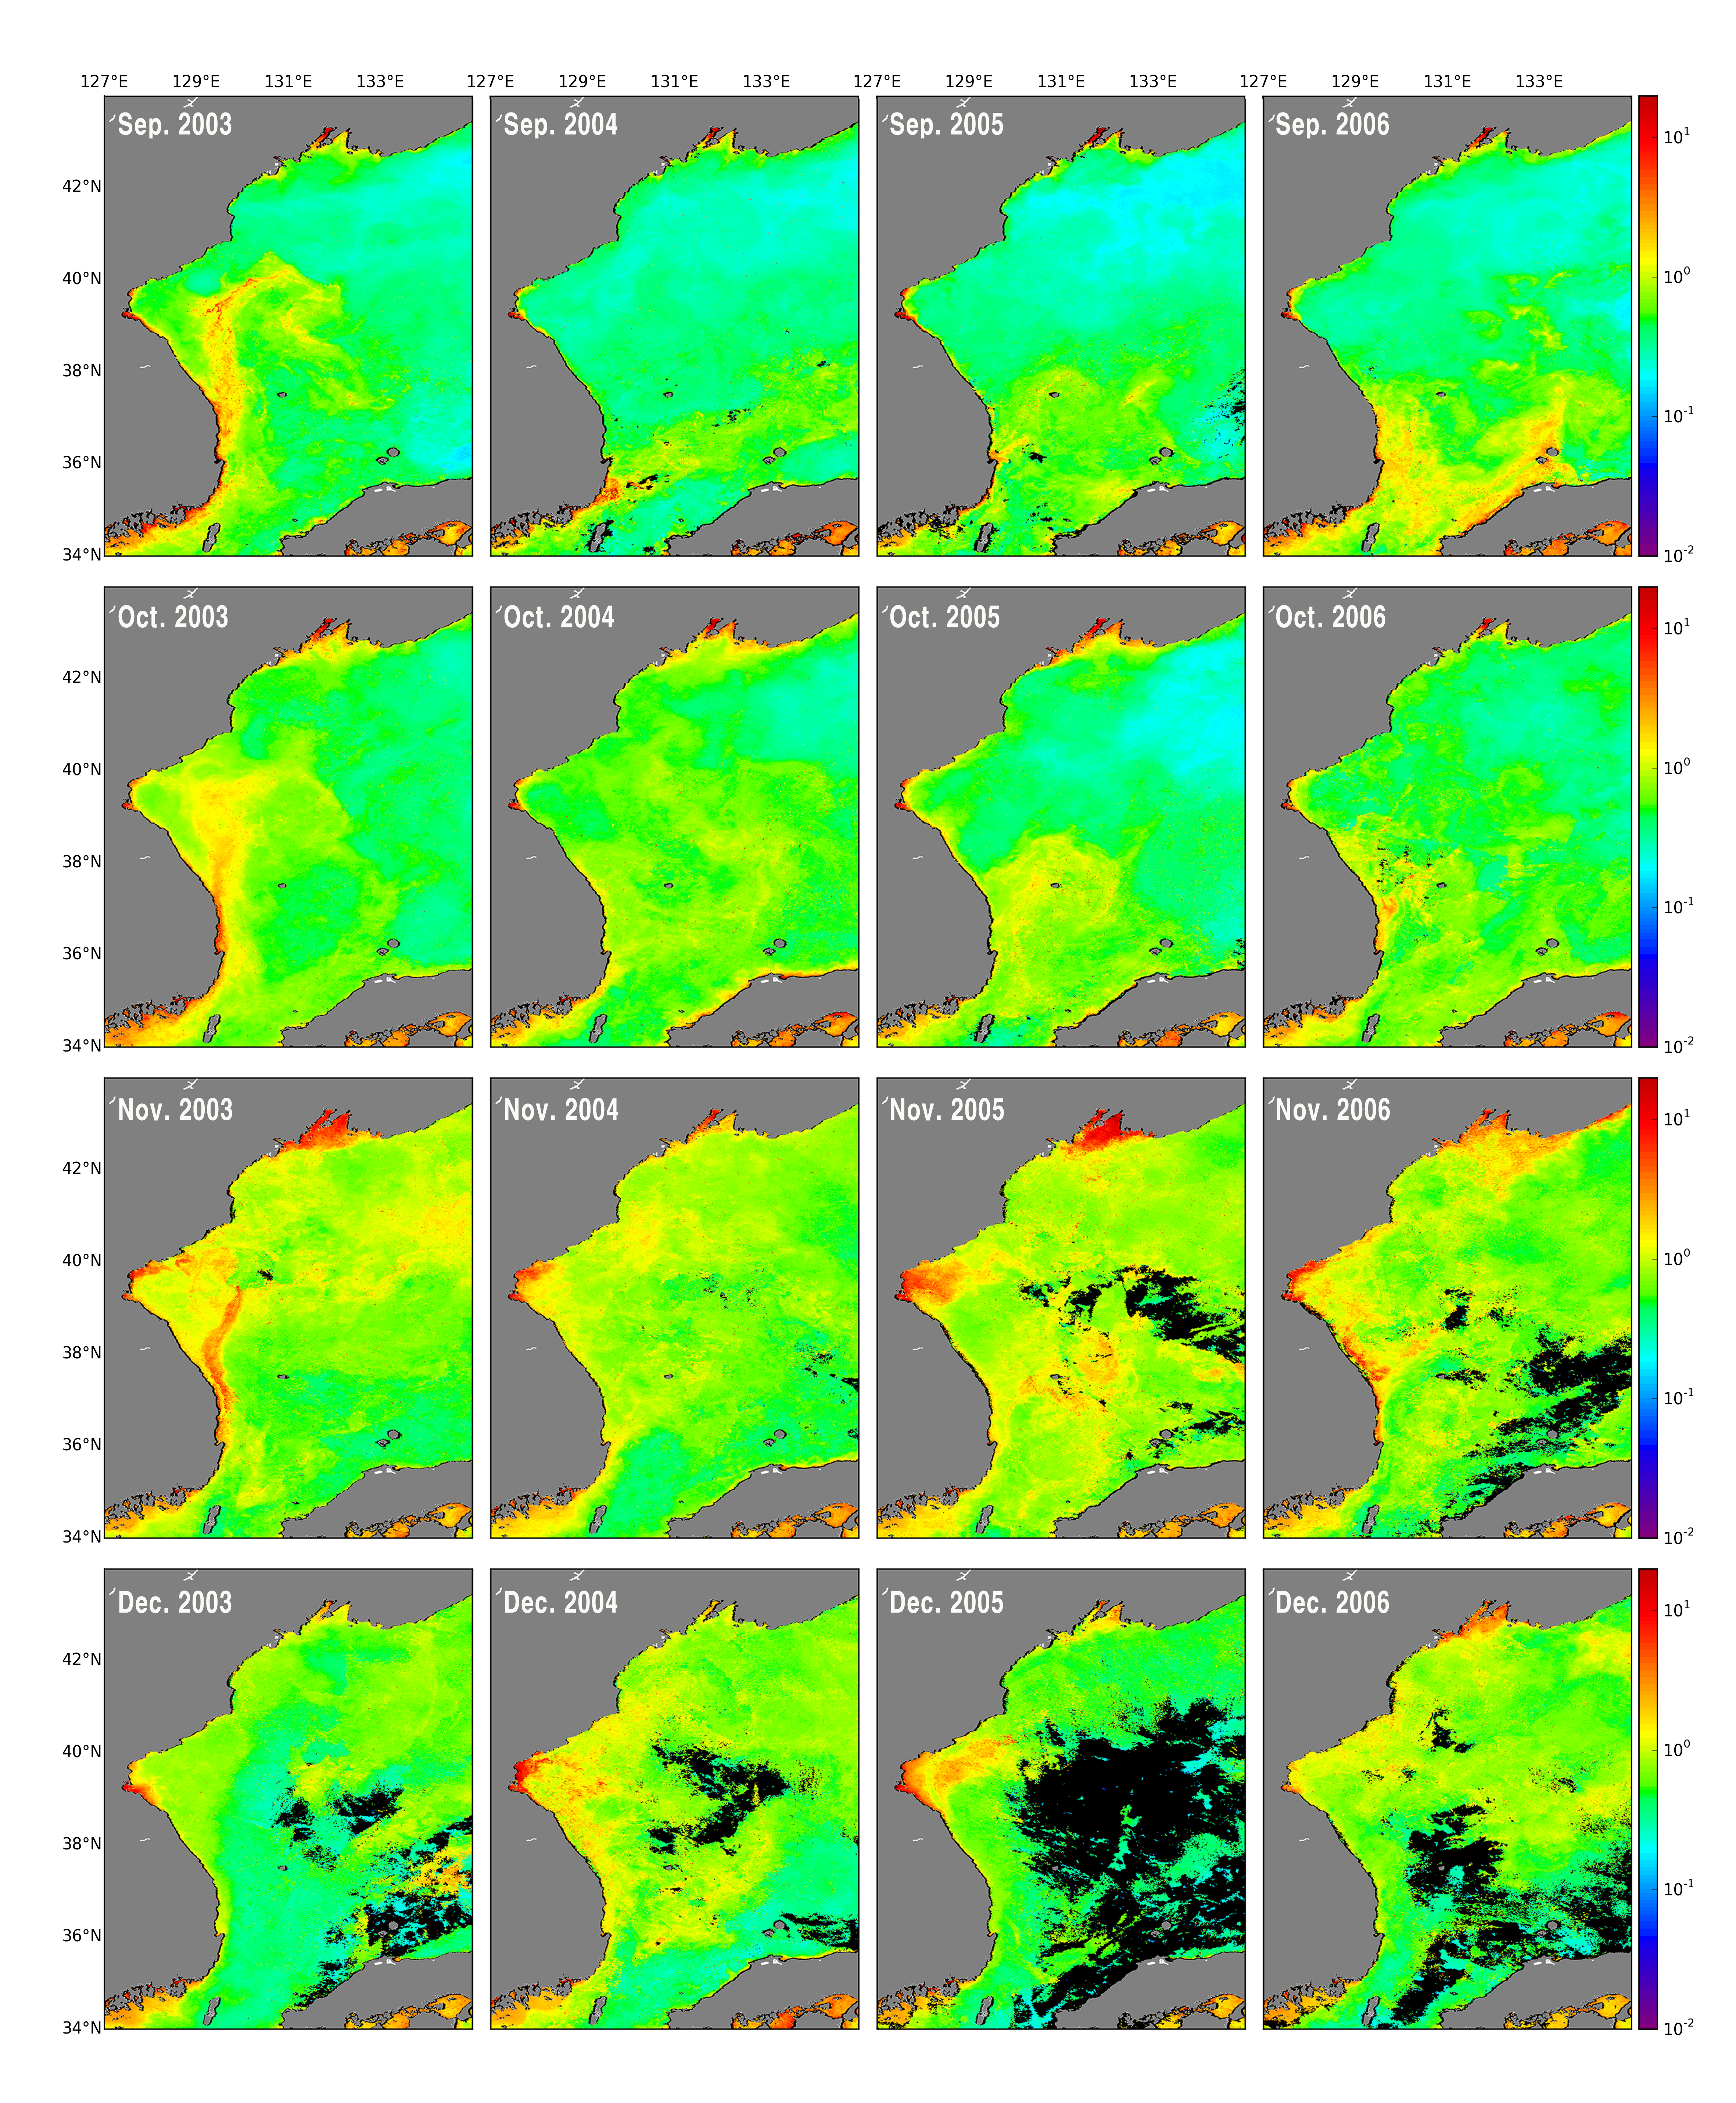
\includegraphics[width=1.00\textwidth]{monLAC03}\\
	\caption{The monthly-mean chlorophyll-a distribution in the East Sea (Sea of Japan), LAC. From 2003 to 2006, September to December.}
	\label{fig:monLAC03}
\end{figure}


\begin{figure}[h]
	\centering
	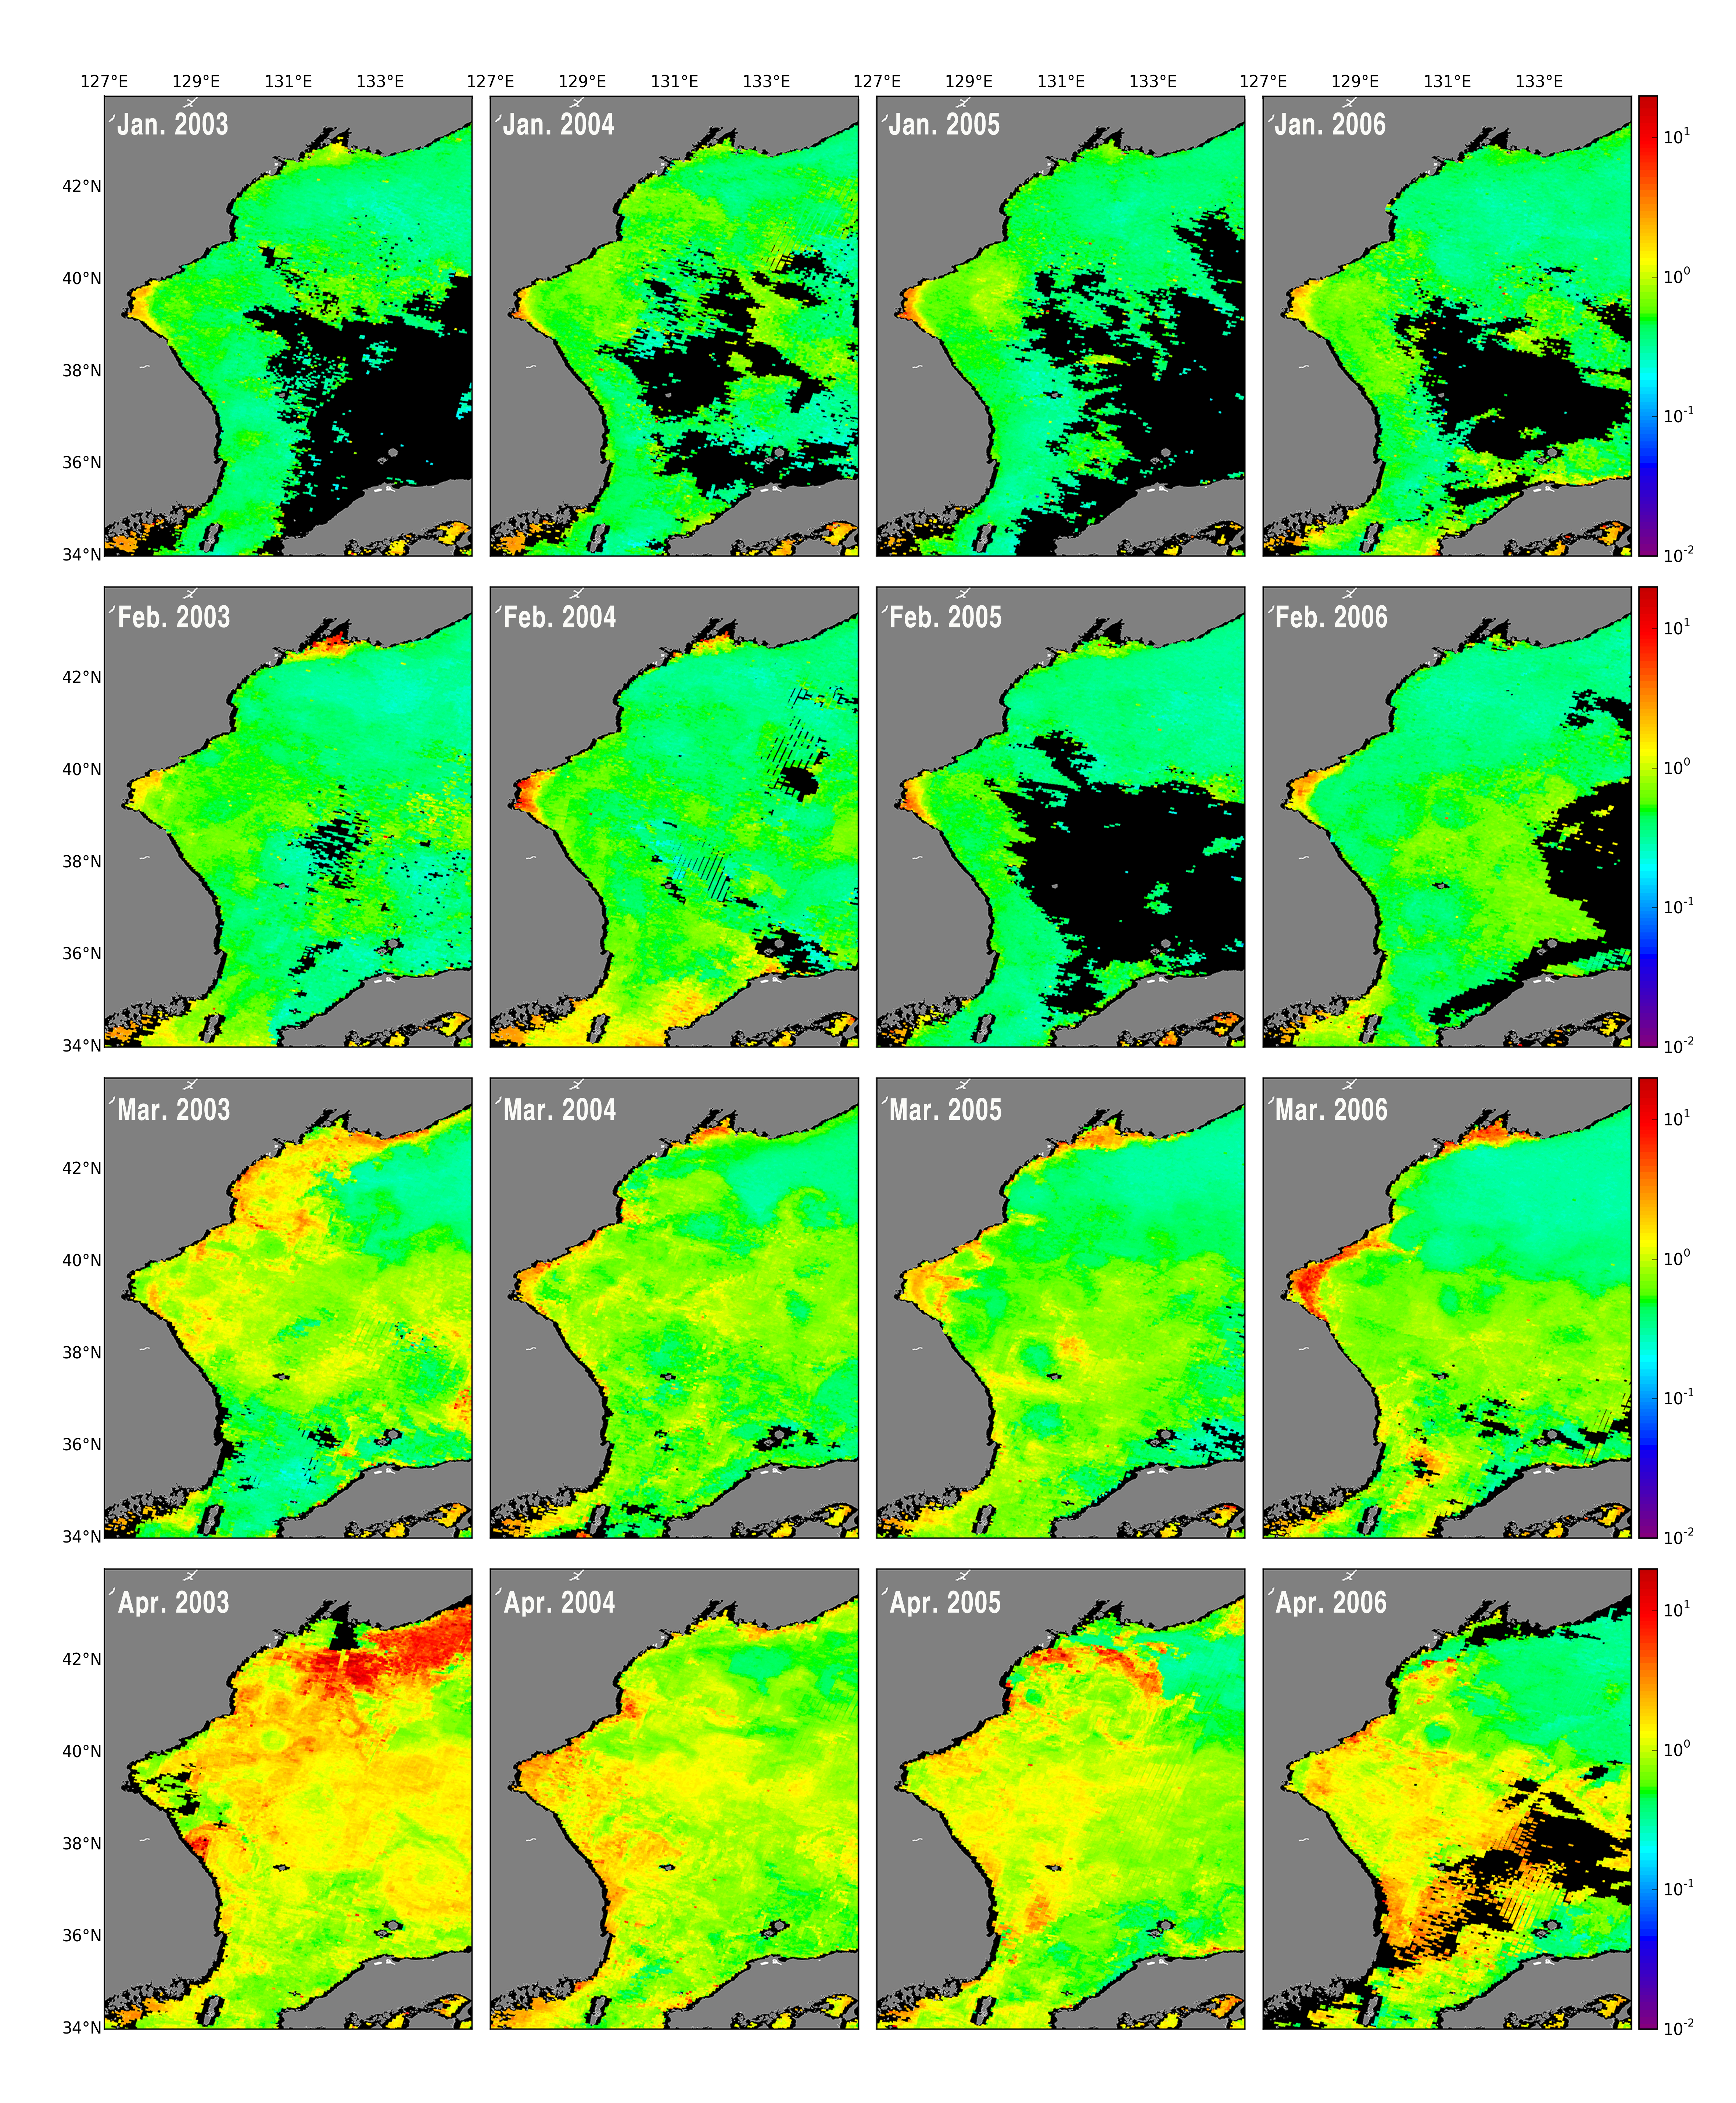
\includegraphics[width=1.0\textwidth]{monGAC01}\\
	\caption{The monthly-mean chlorophyll-a distribution in the East Sea (Sea of Japan), LAC. From 2003 to 2006, January to April.}
	\label{fig:monGAC01}
\end{figure}


\begin{figure}[h]
	\centering
	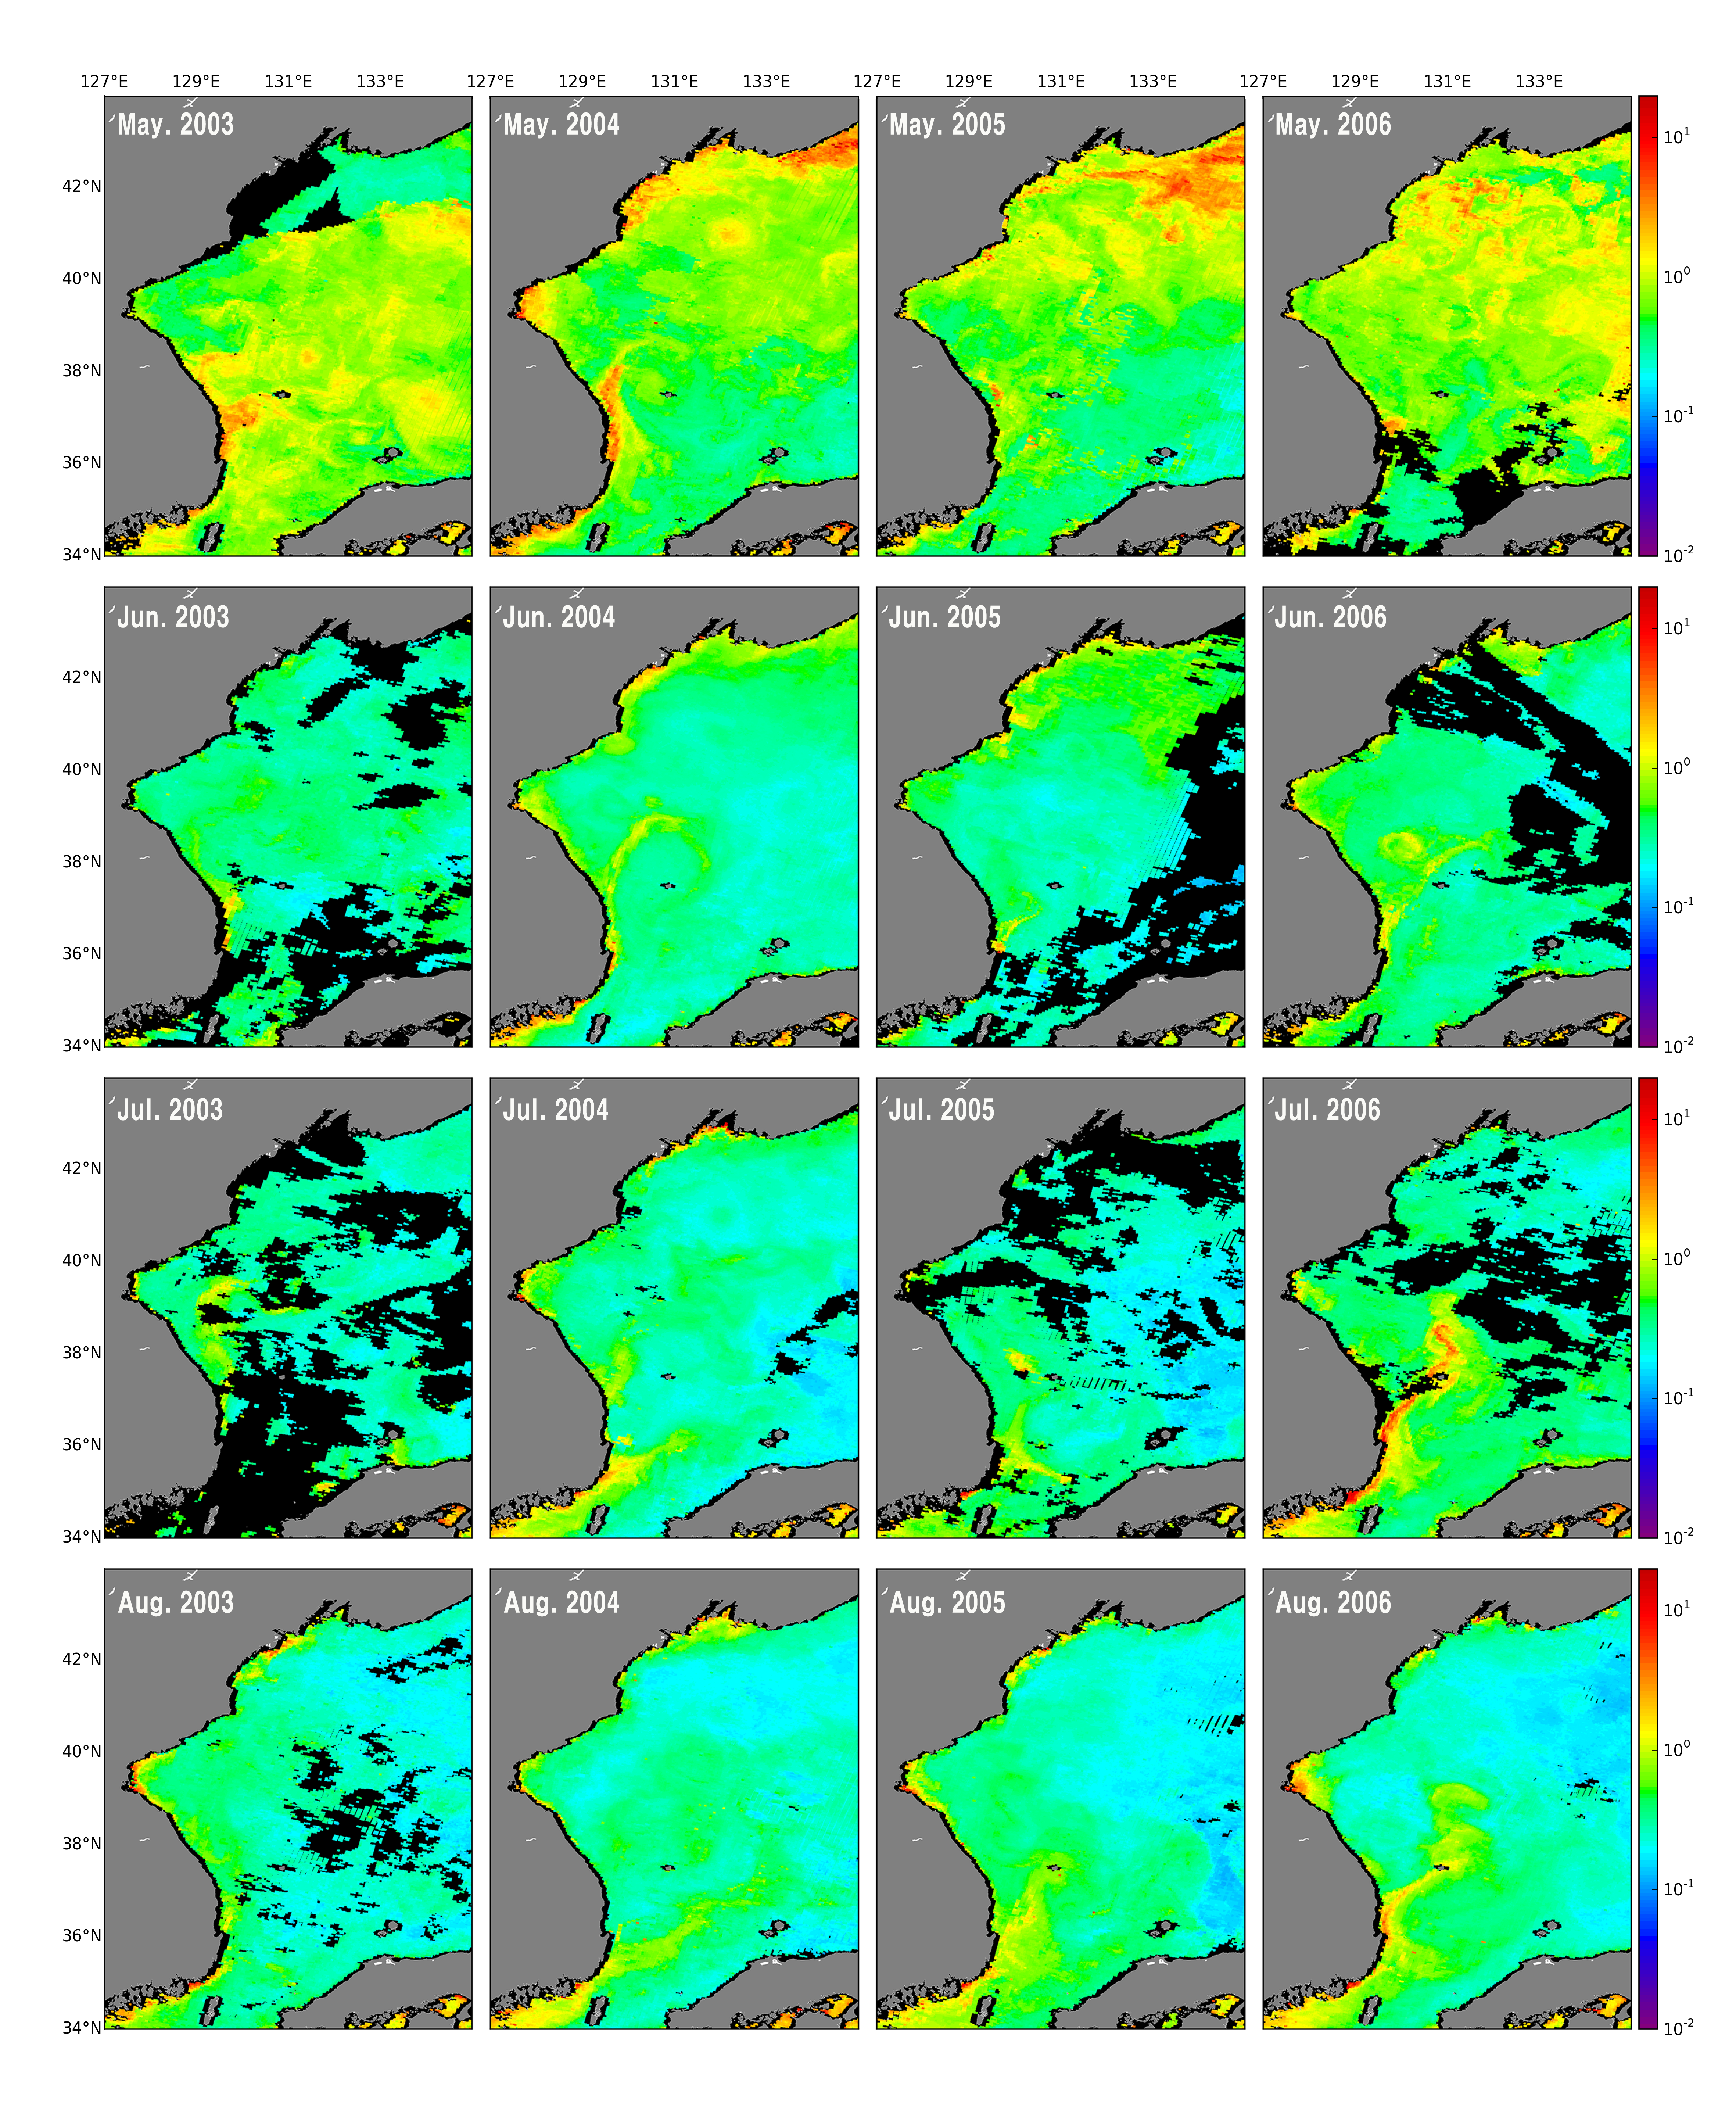
\includegraphics[width=1.00\textwidth]{monGAC02}\\
	\caption{The monthly-mean chlorophyll-a distribution in the East Sea (Sea of Japan), LAC. From 2003 to 2006, May to August.}
	\label{fig:monGAC02}
\end{figure}


\begin{figure}[h]
	\centering
	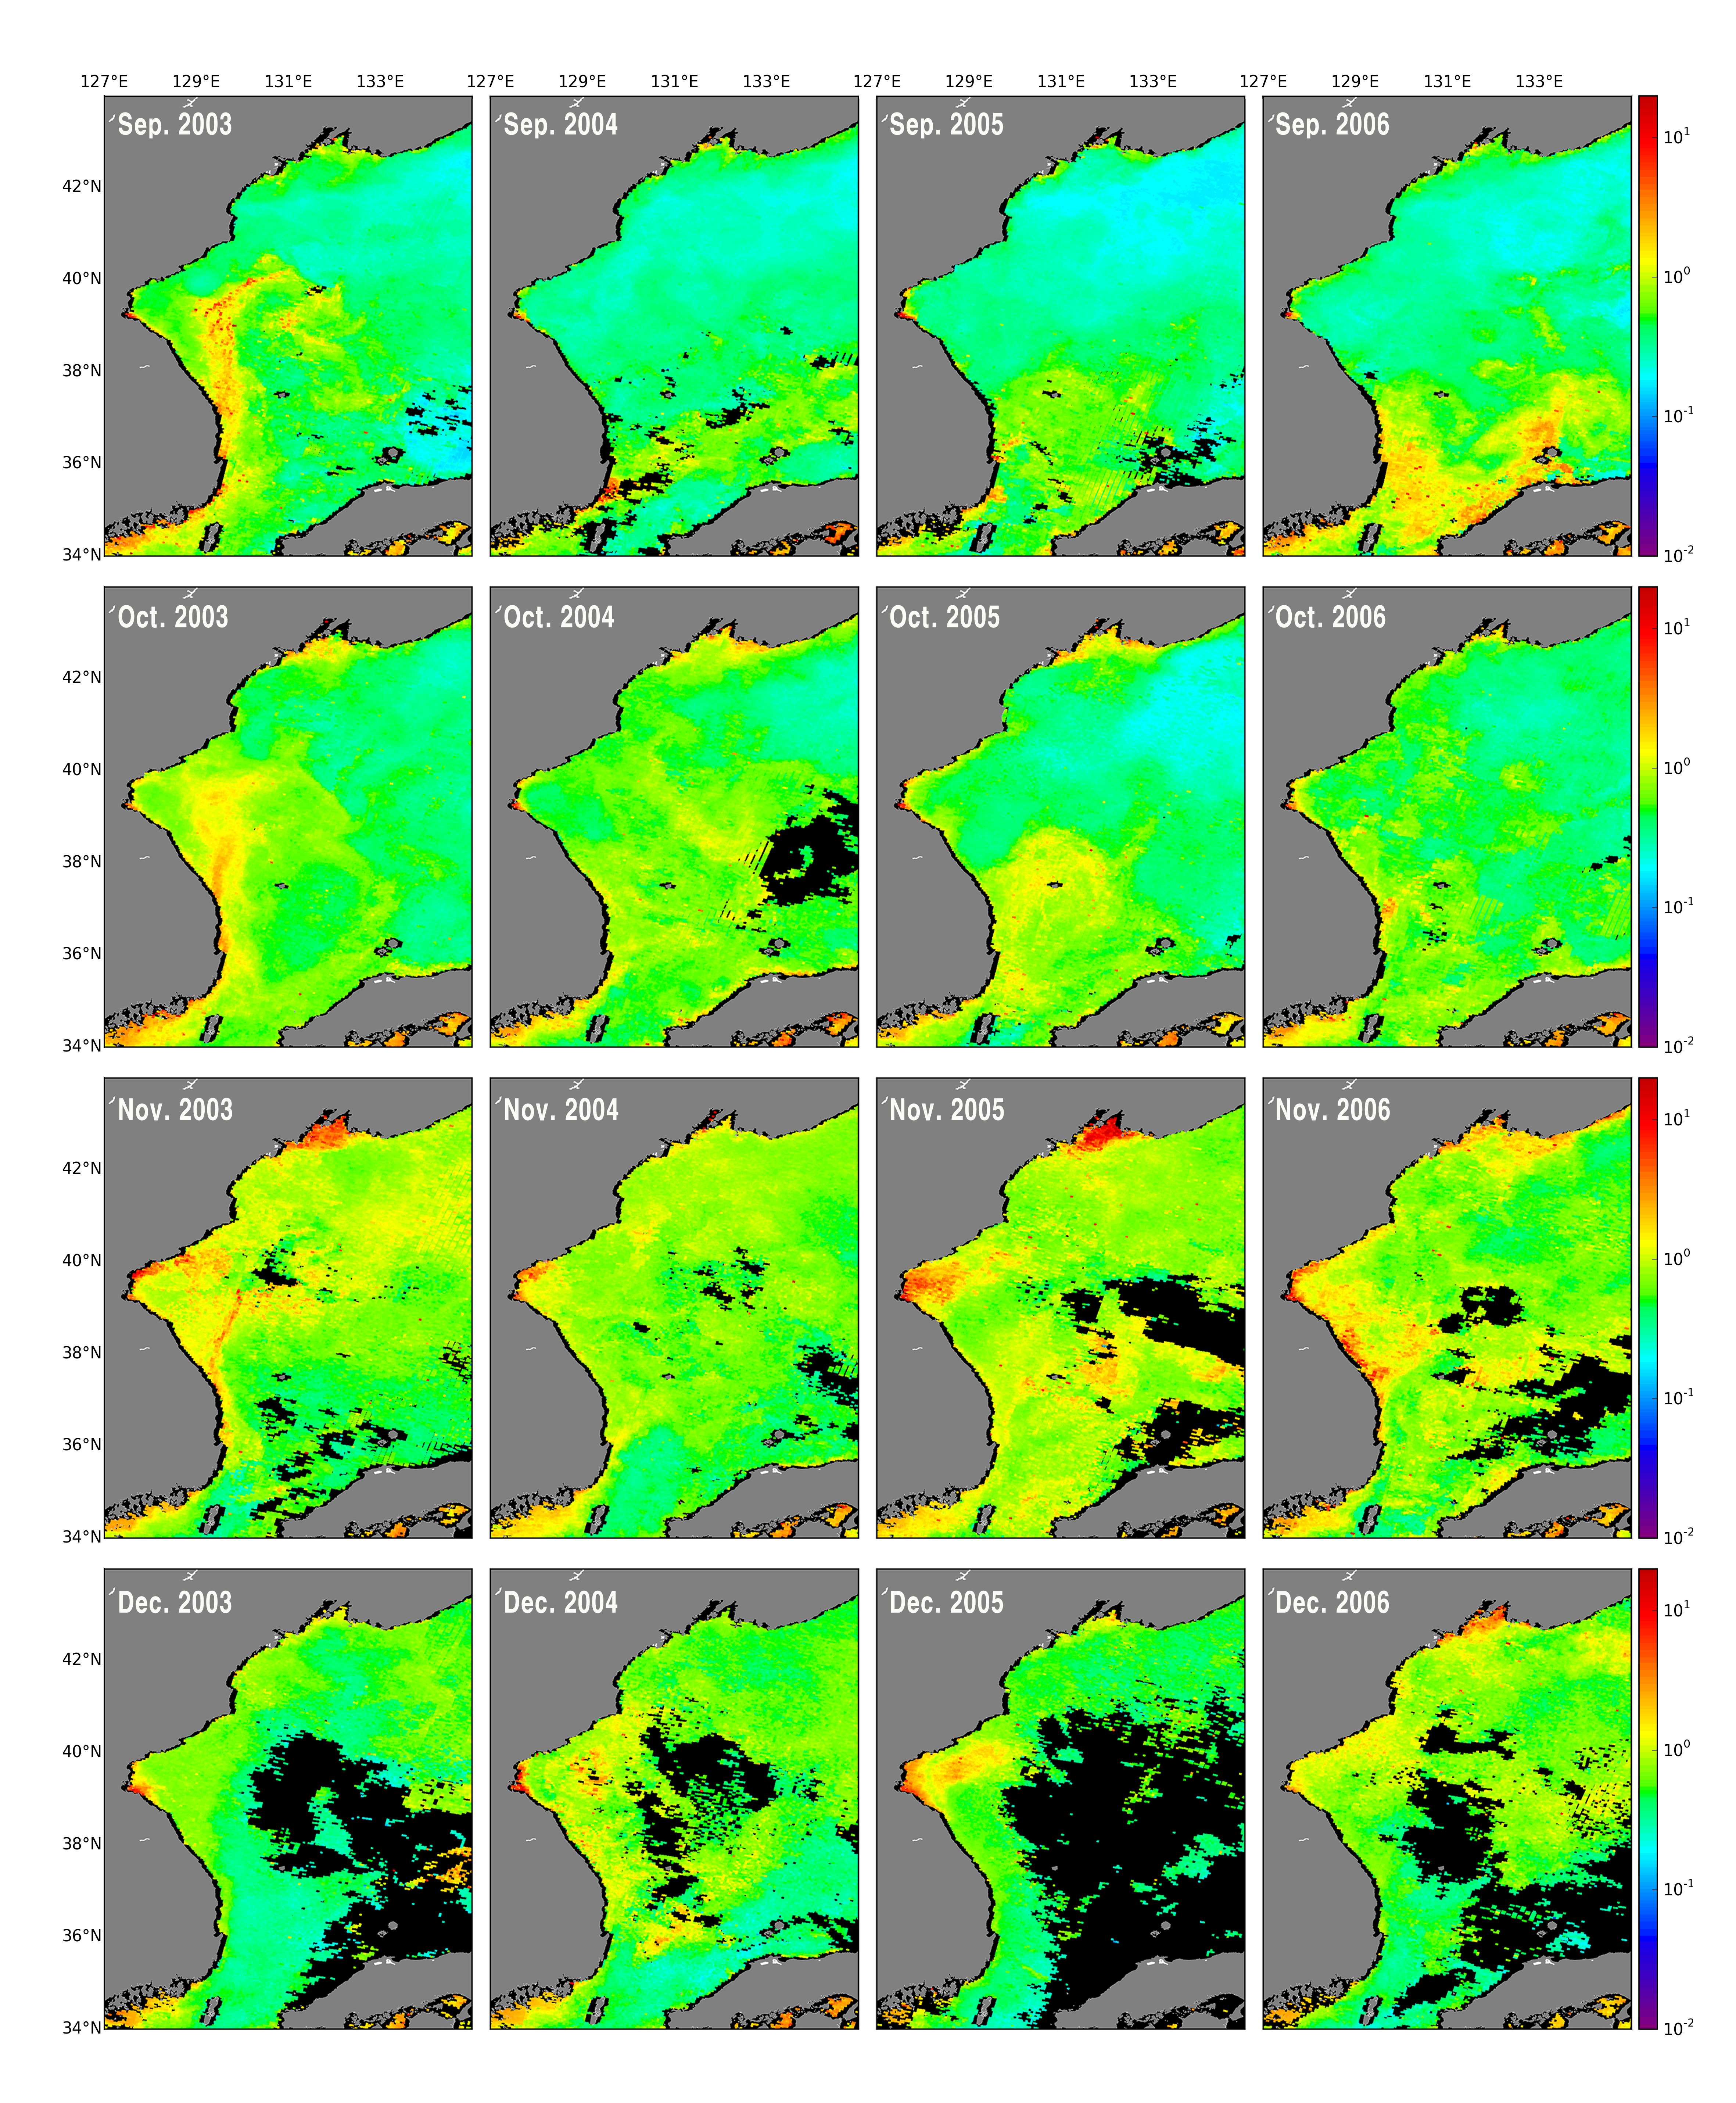
\includegraphics[width=1.00\textwidth]{monGAC03}\\
	\caption{The monthly-mean chlorophyll-a distribution in the East Sea (Sea of Japan), LAC. From 2003 to 2006, September to December.}
	\label{fig:monGAC03}
\end{figure}
